\documentclass[12pt]{article}
\usepackage[margin=0.5in]{geometry}
\usepackage{amsmath,amssymb}
\usepackage[colorlinks=true,linkcolor=blue]{hyperref}
\usepackage{hhline,wrapfig,longtable}
\usepackage{graphicx,listings,mips}
\usepackage{alltt,multicol,scrextend}
\usepackage{upquote}

\pagestyle{empty}
\setlength{\parindent}{0pt}
\graphicspath{{figures/}}
\renewcommand{\ttdefault}{pcr}
\lstset{
    language=[mips]Assembler,
    basicstyle=\footnotesize\ttfamily,
    showspaces=false,
    showstringspaces=false,
    showtabs=false,
    frame=single,
    captionpos=b,
    title=\lstname
}

\begin{document}
\begin{titlepage}
    \centering
    {\Huge \textbf{Pymips}\par}
    {\Large User Guide and Tutorial\par}
    \vfill
    {\textit{Roger Gee}\par}
    \large \today
\end{titlepage}

\tableofcontents
\newpage

\section{Introduction and General Usage}
\label{sec:intro}

Pymips is a simple assembler and simulator platform for MIPS. It is designed to
     be used as a cross-platform tool for exploring assembly language
     programming and building toy compilers. While Pymips doesn't provide a
     complete implementation of the MIPS instruction set, it provides nearly
     everything you would need to implement a basic programming language that
     does integer arithmetic, logic and control branching.

\subsection{Installing Pymips}

Pymips is a Python program and requires Python unless you install the frozen
     version of Pymips. Ideally it should run as a command-line program that can
     be executed by your shell. This means the relevant files should be
     installed in a location defined in the shell's PATH environment
     variable. On POSIX systems this may be a location like
     \texttt{/usr/local/bin}. On Windows you may need to create a directory for
     the program that you add to the shell's \texttt{PATH} environment
     variable. Consult your operating system vendor for the appropriate
     documentation.\\

On POSIX systems, rename \texttt{pymips.py} to \texttt{pymips} when installing
     and ensure the file has executable bits enabled. Note that we do this since
     every invocation example presented in this document will assume the program
     is called \texttt{pymips}.\\

On Windows it is recommended that you install the frozen version so that it can
     be executed more easily as if it were a native binary. If you don't, you
     can execute the \texttt{pymips.py} file directly assuming your Python
     installation has registered \textit{.py} files with the interpreter. This
     allows the shell to launch Python scripts like native binaries.\\

Once you've successfully installed Pymips, you should be able to run the program
     from your shell like so:

\begin{alltt}
    $ pymips ...
\end{alltt}

Alternatively, you can also run the program directly like so:

\begin{alltt}
    $ python pymips.py
        OR (on POSIX systems)
    $ ./pymips.py
\end{alltt}

\textit{But} this becomes burdensome if you work on multiple projects using
     Pymips.

\subsection{Invoking Pymips}

Pymips runs in one of two modes: assembler or simulator. It is also possible to
     run the program through both modes in one step, first in assembler mode
     then in simulator mode. The default mode is simulator, meaning with no
     special arguments Pymips thinks you want to execute a program already
     assembled with Pymips, like so:

\begin{alltt}
    $ pymips program.mips
\end{alltt}

This tells Pymips to execute the assembled program stored in the file
     \textit{program.mips}.\\

To assemble a program from its source assembly instructions, use the
     \texttt{'a'} option to run Pymips in assembler mode. You can also use the
     \texttt{'o'} option in tandem to specify the desired output file for the
     assembled program:

\begin{alltt}
    $ pymips -a program.s -oprogram.mips
\end{alltt}

This command assembles \textit{program.s} into the output file
     \textit{program.mips}. If no input file is specified, Pymips will read from
     its standard input.\\

To see Pymips in action, let's assemble and simulate a simple program that
     prints \textit{Hello World} to the screen. The listing for \textit{hello.s}
     shows a simple program that prints a string to the console:\\

\lstinputlisting[title={{\lstname} - The preeminent first program}]{hello.s}

To assemble the program, run the following command:

\begin{alltt}
    $ pymips -a -ohello.mips hello.s
\end{alltt}

Pymips should have written no output to the screen, which indicates success. The
     file \texttt{hello.mips} now exists and can be executed. Note that the file
     extension \texttt{.mips} is unnecessary. I use it conventionally to refer
     to an assembled MIPS program file. To execute the file, pass it to Pymips
     with no options. You should see the following output:

\begin{alltt}
    $ pymips hello.mips
    Hello, World!
    pymips: error: attempted to execute non-instruction: bad offset in program
\end{alltt}

If you are using a POSIX platform, Pymips will turn on the executable bits of
     the output file's mode. This means you can execute it like any other
     program. This works since Pymips writes a \textit{shebang} into the output
     file that can invoke Pymips. For example:

\begin{alltt}
    $ ./hello.mips
    Hello, World!
    pymips: error: attempted to execute non-instruction: bad offset in program
\end{alltt}

As mentioned earlier, it is possible to have Pymips perform both assembling and
     simulating in one step with the \texttt{'one-step'} option. This produces
     no executable output file and is convenient to use for testing. In this way
     Pymips behaves more like an on-the-fly interpreter than a multistage
     assembler/simulator. For example:

\begin{alltt}
    $ pymips --one-step hello.s
    Hello, World!
    pymips: error: attempted to execute non-instruction: bad offset in program
\end{alltt}

The error message \textit{attempted to execute non-instruction} simply means
     that our simple program didn't exit normally. The next section will explain
     how to write MIPS programs and will eventually address this issue.\\

\newpage
\section{Writing MIPS programs for Pymips}

While this guide assumes you are familiar with MIPS and assembler programming,
     this section provides some important information regarding how to write
     assembly language programs for the Pymips platform. It will also provide
     suggestions on how several high-level programming language features may be
     implemented at the Pymips level.\\

A MIPS program is completely \textit{unstructured}. This means there are no
     innate control mechanisms built into the language's syntax. A program is
     simply a set of instructions (called the \textit{program text}), executed
     one after the other. In addition to a program's instructions are its memory
     segments. The program's main memory is divided into two different segments:
     the \textit{data segment} and the \textit{stack segment}. The program's
     data segment is a region of memory that is used to store global data. The
     stack segment is a memory region used for local data storage. This section
     will explain these different parts of a MIPS program in more detail.

\subsection{MIPS Registers}

Registers are the most basic memory regions in an assembler program. They
     correspond to memory directly available in the CPU. Most instructions
     require that data first be loaded into a register. MIPS has 32 general
     purpose registers, each having one word (i.e. 32 bits) of space. The
     registers have numeric names from \texttt{\$0} to \texttt{\$31} and also
     conventional names. The following table lists the general purpose
     registers, including their numeric and conventional names followed by a
     short description of their conventional use:\\

\begin{tabular}{c | c | c}
    \textbf{numeric name} & \textbf{conventional name} & \textbf{usage}\\
    \hhline{=|=|=}
    \texttt{\$0} & \texttt{\$zero} (\texttt{\$r0}) & holds the value zero \\ \hline
    \texttt{\$1} & \texttt{\$at} & argument temporary register \\ \hline
    \texttt{\$2} & \texttt{\$v0} & return value register \\ \hline
    \texttt{\$3} & \texttt{\$v1} & return value register \\ \hline
    \texttt{\$4} & \texttt{\$a0} & argument register \\ \hline
    \texttt{\$5} & \texttt{\$a1} & argument register \\ \hline
    \texttt{\$6} & \texttt{\$a2} & argument register \\ \hline
    \texttt{\$7} & \texttt{\$a3} & argument register \\ \hline
    \texttt{\$8} & \texttt{\$t0} & temporary register (unpreserved) \\ \hline
    \texttt{\$9} & \texttt{\$t1} & temporary register (unpreserved) \\ \hline
    \texttt{\$10} & \texttt{\$t2} & temporary register (unpreserved) \\ \hline
    \texttt{\$11} & \texttt{\$t3} & temporary register (unpreserved) \\ \hline
    \texttt{\$12} & \texttt{\$t4} & temporary register (unpreserved) \\ \hline
    \texttt{\$13} & \texttt{\$t5} & temporary register (unpreserved) \\ \hline
    \texttt{\$14} & \texttt{\$t6} & temporary register (unpreserved) \\ \hline
    \texttt{\$15} & \texttt{\$t7} & temporary register (unpreserved) \\ \hline
    \texttt{\$16} & \texttt{\$s0} & save register (preserved) \\ \hline
    \texttt{\$17} & \texttt{\$s1} & save register (preserved) \\ \hline
    \texttt{\$18} & \texttt{\$s2} & save register (preserved) \\ \hline
    \texttt{\$19} & \texttt{\$s3} & save register (preserved) \\ \hline
    \texttt{\$20} & \texttt{\$s4} & save register (preserved) \\ \hline
    \texttt{\$21} & \texttt{\$s5} & save register (preserved) \\ \hline
    \texttt{\$22} & \texttt{\$s6} & save register (preserved) \\ \hline
    \texttt{\$23} & \texttt{\$s7} & save register (preserved) \\ \hline
    \texttt{\$24} & \texttt{\$t8} & temporary register (unpreserved) \\ \hline
\end{tabular}\\

\begin{tabular}{c | c | c}
\textbf{numeric name} & \textbf{conventional name} & \textbf{usage}\\
    \hhline{=|=|=}
    \texttt{\$25} & \texttt{\$t9} & temporary register (unpreserved) \\ \hline
    \texttt{\$26} & \texttt{\$k0} & kernel register \\ \hline
    \texttt{\$27} & \texttt{\$k1} & kernel register \\ \hline
    \texttt{\$28} & \texttt{\$gp} & global pointer register \\ \hline
    \texttt{\$29} & \texttt{\$sp} & stack pointer register \\ \hline
    \texttt{\$30} & \texttt{\$fp} & frame pointer register \\ \hline
    \texttt{\$31} & \texttt{\$ra} & return address register \\ \hline
\end{tabular}

\vspace{0.1in} Some of these registers (e.g. \texttt{\$k0}, \texttt{\$k1}) have
     no special use since Pymips is only a simulator. So you can use them for
     whatever purpose you deem fit. Note that even though a register has a
     conventional use, you can disregard it and still have a valid assembly
     program.

\subsection{Formatting Instructions}

Instructions belong in the program's text segment. To indicate to the assembler
     that we want to place instructions in the program's text, we use the
     \texttt{.text} directive\footnote{A \textit{directive} is a statement in an
     assembler program that indicates some metainformation about the
     program. They always begin with a dot (\texttt{.}).}. The basic format of a
     program should be as follows:

\begin{alltt}
    .text
    [instructions follow...]
\end{alltt}

Instructions have a simple syntax to follow. Each instruction is represented by
     a text label (e.g. \texttt{add} or \texttt{move}). The instruction's
     arguments (if any) follow the instruction label and are
     comma-separated. The following example listing demonstrates some
     instructions that print out the integer 4:

\begin{lstlisting}
    .text
    li $a0, 4 # load 4 into register
    li $v0, 1 # load 1 (print_int)
    syscall   # system call to print integer
\end{lstlisting}

A full listing of supported instructions and their syntax is available in the
     \hyperref[sec:iref]{instruction reference} section.

\subsection{System Calls}

To make any useful MIPS program, we need to interact with the system
     (e.g. reading input, writing output). To do this, the simulator provides
     system calls. A system call is a special instruction that breaks to a
     procedure executed by the system (which in this case is the Pymips
     simulator). The following table details the available system calls
     supported by Pymips:\\

\begin{tabular}{p{0.15\textwidth} || p{0.025\textwidth} | p{0.275\textwidth} | p{0.45\textwidth}}
    \textbf{syscall} & \textbf{no.} & \textbf{arguments} &
     \textbf{description} \\ \hhline{=#=|=|=}

    \texttt{print\_int} & 1 & \texttt{\$a0} - word to print & Print an integer
     to stdout \\ \hline

    \texttt{print\_string} & 4 & \texttt{\$a0} - pointer to null-terminated
     string & Print a text string to stdout \\ \hline

    \texttt{read\_int} & 5 &  & Returns next input token interpreted as an
     integer \\ \hline

    \texttt{read\_string} & 8 & \texttt{\$a0} - pointer to input buffer;
     \texttt{\$a1} - size of input buffer & Reads a string into the input buffer
     up until a newline character, the end of input or until the buffer is
     full\footnote{if a newline character is read, it will be read into the
     buffer}; returns the number of bytes read \\ \hline
\end{tabular}

\begin{tabular}{p{0.20\textwidth} || p{0.025\textwidth} | p{0.275\textwidth} | p{0.40\textwidth}}
    \textbf{syscall} & \textbf{no.} & \textbf{arguments} &
     \textbf{description} \\ \hhline{=#=|=|=}

    \texttt{exit} & 10 & \texttt{\$a0} - process return code & Terminate the
     process (this should be done at the end of every well-formed program)
     \\ \hline

    \texttt{print\_character} & 11 & \texttt{\$a0} - character to print & Print
     single character; the argument should be in the range $0..255$ \\ \hline

    \texttt{read\_character} & 12 & & returns the next character read from stdin\\
\end{tabular}

\vspace{0.25in}
To make a system call, use the \texttt{syscall} instruction. The value of the
     \texttt{\$v0} register determines which system call to execute and is
     called the \textit{system call number}. Any arguments to system calls are
     passed in using the argument registers (\texttt{\$a0 .. \$a3}). If a system
     call returns a value, it places it in the \texttt{\$v0} register.\\

It's worth mentioning the purpose of the \texttt{exit} system call as it is
     actually very important. Most operating systems require that a process call
     an exit-like system call to terminate normally. When calling exit, you must
     pass a value between 0 and 255 for the process's termination status. A
     value of 0 typically means the process exited without any errors. This is
     an important runtime task typically preformed in a C/C++ program after
     \texttt{main} returns. For more details, see the
     \hyperref[sec:runtime]{section on writing runtime functionality}.

\subsection{Formatting the Data Segment}

Obviously space in the registers is limited and more memory is required. The
     data segment is the part of a program's main memory that allows you to
     allocate storage locations that can be accessed globally. Data segment
     directives allow you to place specific values into main memory that are
     available at runtime (e.g. a text string). Any data segment directive must
     follow an initial \texttt{.data} directive. You can place these directives
     anywhere in the program and mix them with \texttt{.text} directives however
     you choose.\\

Pymips supports the following data directives:\\

\begin{addmargin}[0.5in]{0.5in}
    \texttt{.byte <N>, [<N>, <N>, ...]} - define a byte\\
    \texttt{.half <N>, [<N>, <N>, ...]} - define a half-word (i.e. 2-byte value)\\
    \texttt{.word <N>, [<N>, <N>, ...]} - define a word (i.e. 4-byte value)\\
    \texttt{.ascii <STRING>} - define ASCII string\\
    \texttt{.asciiz <STRING>} - define zero-terminated ASCII string\\
    \texttt{.space <AMOUNT>} - define arbitrary block of memory\\
\end{addmargin}

The directives \texttt{.byte}, \texttt{.half} and \texttt{.word} allow you to
     specify one or more literal integer values to place in the data
     segment. The rest of the data segment directives expect only a single
     value. The argument to the \texttt{.space} directive is the number of bytes
     you wish to allocate. When using the \texttt{.ascii} or \texttt{.asciiz}
     directives you give a string literal (double-quoted text string). You can
     use special escape sequences inside the string literals. The standard C
     escape sequences are supported, including octal and hexadecimal
     literals. Octal literals contain three digits and hex literals contain two
     digits following the backslash. For example the following are all
     equivalent:\\

\begin{addmargin}[0.5in]{0.5in}
    \begin{alltt}
        "Hello\textbackslash012" <=> "Hello\textbackslash0a" <=> "Hello\textbackslash\,n"
    \end{alltt}
\end{addmargin}

As a simple example of how the data segment can be used, here is a program that
     prints out a list of numbers stored in its data segment. Notice that an
     extra address is allocated to detect how long the list is (i.e. denote the
     end):\\
\newpage
\lstinputlisting[title={{\lstname} - Print list of words}]{print-list.s}

Here is another example program that reads in two half-words and prints out the
     value of the resulting word. The first half-word will be the lower 16 bits
     and the second will be the upper 16 bits:

\lstinputlisting[title={{\lstname} - Show transaction with data segment}]{halves.s}

As seen in the example programs, to access data declared in the data segment,
     you use a label\footnote{A label is an identifier that appears first on a
     line in an assembler program followed by a colon (:)}. The label can be
     used with certain instructions and is substituted with the data value's
     address in memory when the program is assembled. Using labels is useful but
     not required when using the different data directives.\\

Note that the data segment in Pymips is only as large as you make it. The first
     data directive gets the lowest magnitude address and every subsequent entry
     is allocated contiguously from there. Pymips will pad the data segment to
     some multiple of eight bytes (for alignment purposes).

\subsection{Understanding the Stack Segment}

Like the data segment, the stack segment is a memory region that is used for
     storing data in the program's main memory. Unlike the data segment, the
     stack segment is used to store local as opposed to global data. This
     distinction makes sense when you consider how procedures are implemented in
     a computer program (think function-local variables instead of global
     variables). Consider the following C program:\\

\begin{lstlisting}[language=C]
#include <stdlib.h>

int a;
int main(int argc,const char* argv[])
{
    int b;

    b = atoi(argv[1]);
    a = b+1;
    return 0;
}
\end{lstlisting}

If this program were compiled to assembler instructions, the variable \texttt{a}
     would be stored in the data segment and the variable \texttt{b} would be
     stored in the stack segment. Furthermore, the parameters \texttt{argc} and
     \texttt{argv} as well as the argument passed to \texttt{atoi} are also
     allocated on the stack.\\

An important feature of stack memory is that it can grow and shrink according to
     the behavior of a stack. Consider a recursive C function that computes a
     factorial:\\

\begin{lstlisting}[language=C]
int fac(int n)
{
    if (n <= 2)
        return (n > 0) ? n : 1;
    return n * fac(n-1);
}
\end{lstlisting}

Each time a call is made to \texttt{fac}, more memory is allocated on the stack
     to store the parameter \texttt{n}. Then, each time \texttt{fac} returns,
     the memory is ``popped off'' so to speak. As you can tell, this is an
     important feature for making sure we have unique memory locations for each
     instantiation of a procedure.\\

Stack memory is addressed by the value of the stack pointer register,
     \texttt{\$sp}\footnote{Note that there is also a frame pointer
     \texttt{\$fp} register that is used for addressing the stack}. Unlike the
     data segment, where we have hard-coded labels that represent memory
     locations, the stack is addressed solely by means of the stack pointer
     register (and offsets from that register).\\

Stack memory always grows \textit{downwards}. When a program begins, the stack
     pointer contains the highest possible address available on the stack. This
     means that the most recently allocated address should be that with the
     lowest magnitude. To allocate more data on the stack, simply subtract from
     the stack pointer by the number of bytes you wish to allocate.\\

Obviously the stack can run out of space if it grows too much. Eventually the
     stack segment and data segment collide given Pymips' memory layout. This
     means you could potentially overwrite the data segment if your program
     pushes past the stack segment. Pymips doesn't check for actual stack
     overflows, just if you push out of the total available main memory. Note
     that Pymips gives 1MB of space to the stack.\\

The next section will show practical uses of the stack in implementing
     procedures.

\subsection{Procedures}
\label{sec:proc}

A procedure is a reusable block of instructions that fulfills some purpose
     within the program. This corresponds to the concept of a function in
     C. However, unlike in C, assembler programming is still unstructured,
     meaning there are no assembly language constructs that innately support
     procedures. Instead, a procedure is defined (like many things in assembler
     programming) conventionally. This means that we could define our own
     convention if we wanted. However, in this guide, we are going to explore a
     common calling convention used to implement procedures in MIPS assembler
     programs.\\

The first thing to understand about a procedure is that it is just a block of
     instructions to which the program will jump. Once executed, we jump back to
     the address from which the procedure was called. To do this, we use the
     \texttt{jal} and \texttt{jr} instructions. When \texttt{jal} is executed,
     it saves the current offset in the program text to the register
     \texttt{\$ra} and jumps to the specified offset. The instruction
     \texttt{jr} allows us to jump to the address as specified in a register; in
     this case this will be the \texttt{\$ra} register set by \texttt{jal}.\\

The basic outline of a procedure would look like the following:\\
\begin{lstlisting}
proc:       # beginning of procedure
    ...     # some useful instructions
    jr $ra  # return back to caller
\end{lstlisting}

To call this procedure, we would issue the following instruction: \texttt{jal
     proc}.\\

Defining the body of and calling a procedure is pretty easy. Unfortunately
     procedures introduce some more complexity we have to worry about such as
     arguments, return values and local data storage. We also have to worry
     about potentially overwriting any registers that are in use between
     procedure calls. Fortunately, the calling convention is detailed enough to
     consider all of these scenarios so that we can take appropriate
     action. Since all of these details involve the stack, let's start by
     discussing the layout of the stack.\\

Figure \ref{fig:stackframe} shows a generic MIPS stack frame according to the C
     calling convention. A \textit{stack frame} is a block of contiguous memory
     on the stack that is used locally by a procedure. When a procedure begins,
     it updates the stack pointer register to point to the top of its new stack
     frame. In this case, the ``top'' of the stack is what \texttt{\$sp} points
     to in the figure (the bottom of the figure). Each stack frame is allocated
     to some multiple of 8-bytes to avoid address-alignment errors\footnote{This
     is why there is an empty space above \textit{return address} in the stack
     frame diagram; this can represent zero or more words of padding to help
     achieve alignment. Alignment ensures that objects placed on the stack have
     addresses that are easily computed (e.g. some multiple of a power of two).}
      (for objects of up to size 64-bits). If your source language only uses
     data objects that are at most a word size long then you could get away with
     using multiples of four but this guide will show examples that allocate to
     a multiple of eight.\\

\begin{wrapfigure}{r}{0.55\textwidth}
\centering
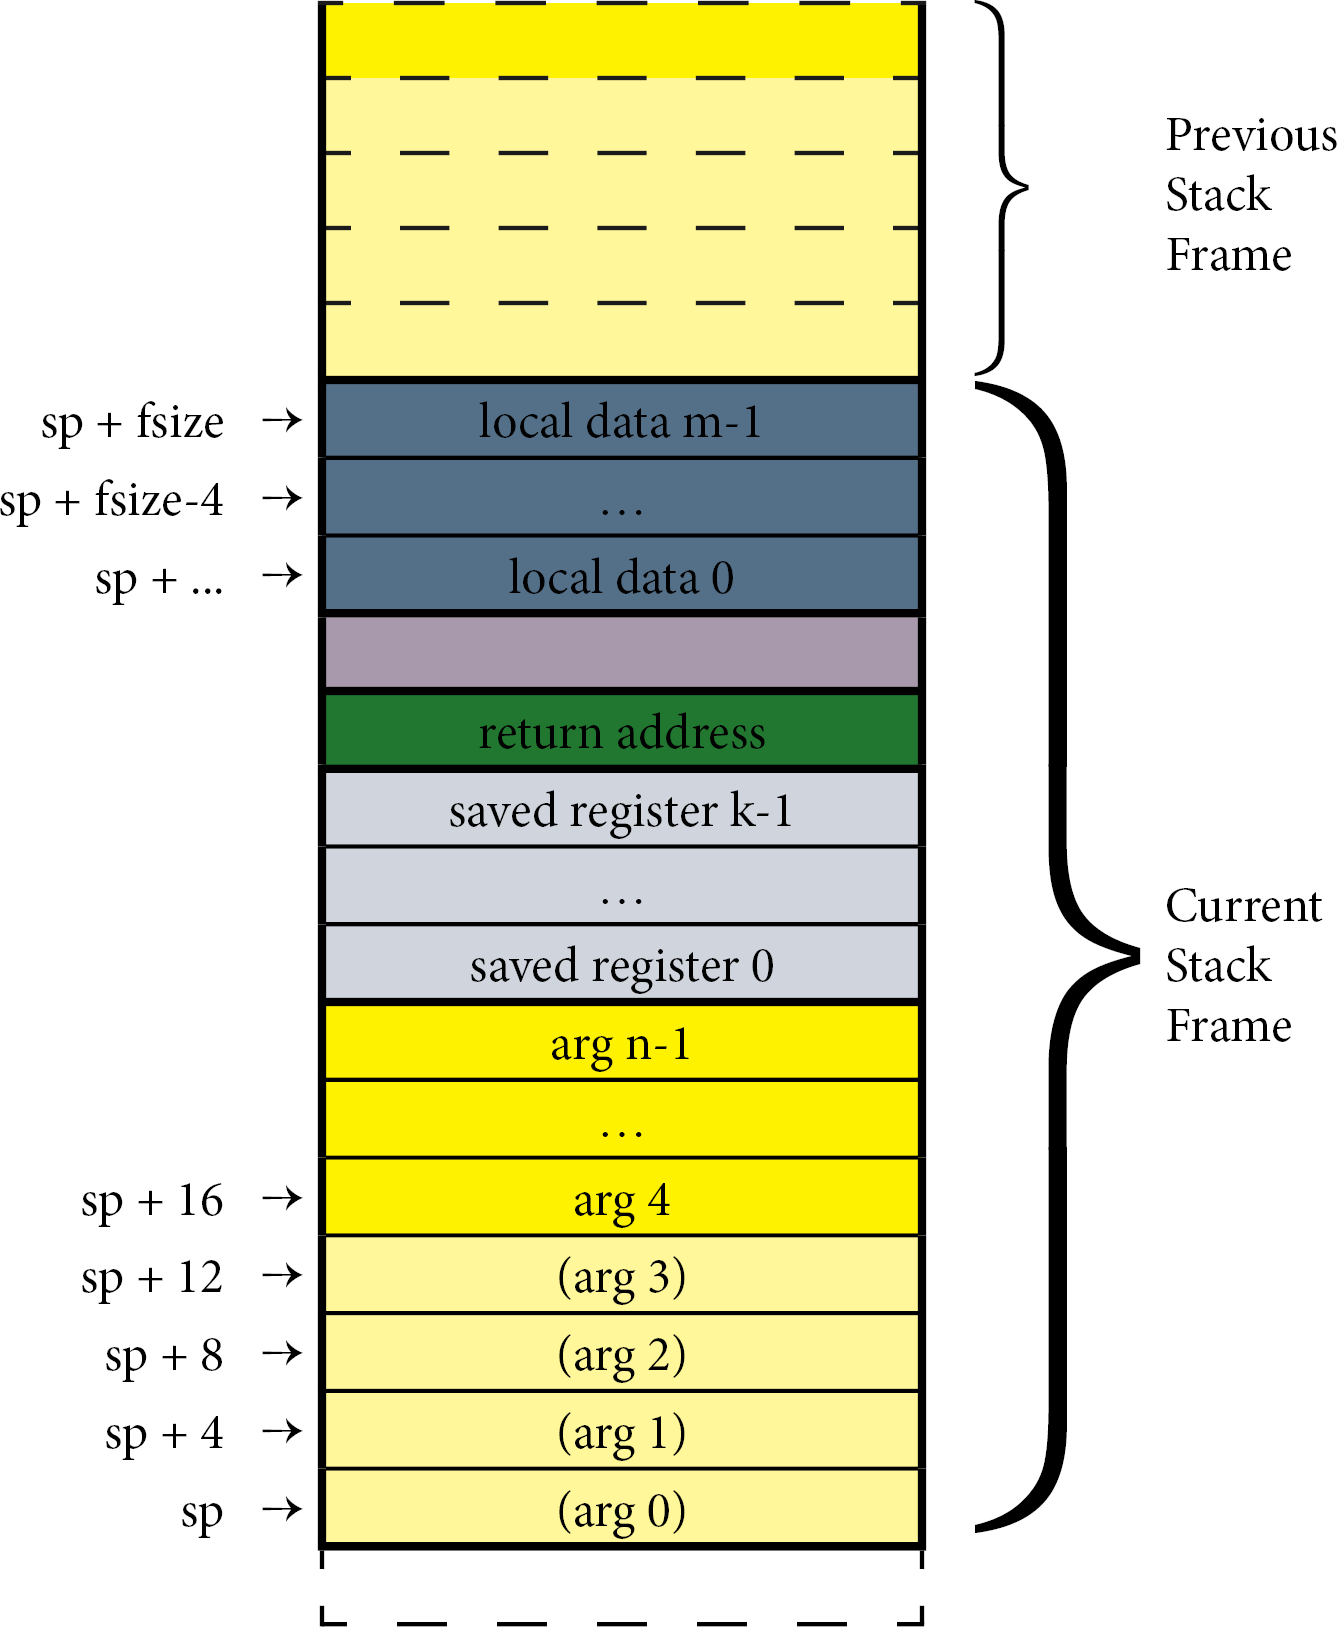
\includegraphics{stack-frame.png}
\caption{A MIPS stack frame}
\label{fig:stackframe}
\end{wrapfigure}

Notice that the stack frame has storage for all the things we mentioned
     earlier. But, as you may have realized, not every procedure will need all
     these things. For example, a procedure may not require any argument space
     if it never makes a procedure call of its own (a so-called \textit{leaf
     procedure}). Also consider a procedure that doesn't require any stack space
     (i.e. it doesn't need a stack frame at all). The rule of thumb to remember
     is that if something is omitted it shouldn't change the order of sections
     in the generic stack frame specification. An omission simply gives a
     section a size of zero.\\

The following subsections will give more specific information and examples on
     using the different parts of the stack frame.\\

\subsubsection{Return Address}

A procedure needs to remember the address of its caller so that it can
     return. When it is called this address is stored in the \texttt{\$ra}
     register. If a procedure makes a procedure call itself this value will be
     overwritten. Therefore we must save this value on our stack frame. Space
     for the return address is positioned below the local variable space. A
     procedure will commonly write the return address to the stack just after
     allocating its stack frame. Before the procedure returns it will restore
     the value of \texttt{\$ra} from the stack frame. If the procedure does not
     make a procedure call itself, there is no need to save the return address
     to the stack.\\

Here is a quick example of saving/restoring the return address:
\begin{lstlisting}
proc:   addiu   $sp, $sp, -24   # 16 bytes for arguments + 8 bytes
        sw      $ra, 16($sp)    # store return address above arguments

        ...                     # do some stuff

        lw      $ra, 16($sp)    # restore return address
        addiu   $sp, $sp, 24    # pop off stack frame
        jr      $ra
\end{lstlisting}
\vspace{-0.25in}
\subsubsection{Return Value}

A procedure should store its return value in the register \texttt{\$v0}. If you
     need more space for a return value, you can also use the register
     \texttt{\$v1}. If you need to return a compound data type from a procedure,
     you would need to allocate space in the caller's stack frame (this exceeds
     the scope of this guide).

\subsubsection{Save Registers}
\label{sec:saveregs}

The calling convention specifies certain registers (i.e. the save registers,
     \texttt{\$s0 .. \$s7}) to be saved to the stack by a procedure. A procedure
     only saves a register if it intends to modify its value. In this way, we
     only go through the expense of saving and restoring a register if we know
     its value is going to change locally within the procedure. Also note that
     it is the callee's responsibility to save registers, since it knows if it
     is going to modify them.\\

This process works similarly to how the return address register is saved to the
     stack. When the procedure is called, it writes any save registers it will
     use to its stack frame. When the procedure is about to return, it restores
     the original value of these registers. In this way, the caller never is
     aware that they were modified (i.e. the entire process is transparent to
     the caller). A practical example of saving registers is demonstrated in the
     next subsection.

\subsubsection{Arguments}

The most important thing to know about arguments in MIPS is that the four
     argument registers (\texttt{\$a0 .. \$a3}) are used to pass values to
     procedures. Of course, a procedure may require more than four arguments, in
     which case the stack is used to pass in the extra arguments.\\

A procedure's parameters are allocated by its caller and therefore exist in the
     caller's stack frame. The caller \textit{always} allocates space for the
     argument registers (i.e. 16 bytes), even if it passes fewer than four
     arguments. Furthermore it does not write any data into this space. It
     simply provides the callee with some space in case it needs to save the
     values of the argument registers. This is important if the procedure is
     going to invoke another procedure itself which would overwrite the argument
     registers. Any more arguments are written directly to the stack by the
     caller.\\

To access parameters on the stack, we use positive offsets from the bottom of
     our stack frame\footnote{It is possible to use the stack frame register to
     refer to the bottom of our stack frame so that we just have to remember
     offsets from that point on. However, the frame pointer register's purpose
     is difficult to place. Some documentation on MIPS doesn't even specify a
     frame pointer register; instead, register \texttt{\$30} is another save
     register.}. Since the stack pointer points to the top of our stack frame,
     we will need to skip over our stack frame and push into the caller's stack
     frame.\\

Here is a practical example. Consider the following C program that recursively
     computes the $N^{th}$ Fibonacci term (note that any system call wrappers
     implied by the source code denote direct system calls and not procedure
     calls):\\

\newpage
\begin{lstlisting}[language=C]
int fib(int n)
{
    if (n <= 1)
        return n;
    return fib(n-1) + fib(n-2);
}

int main()
{
    print_integer(fib(read_integer()));
    print_character('\n');
    return 0;
}
\end{lstlisting}

Since we make two recursive calls that depend on parameter \texttt{n}, we will
     have to save the value of \texttt{n} on the stack so that we can recall it
     after making the first recursive call. We also have to save the return
     value of the first recursive call. We'll use the
     \hyperref[sec:saveregs]{save register} \texttt{\$s0} for this purpose.\\

Each call to \texttt{fib} will allocate 24 bytes on the stack since we must
     allocate at least 4 words for argument space plus some space for the return
     address and save registers (this procedure uses no local variables). The
     argument stack space will be used by \textit{both} the first and second
     recursive calls.\\

\newpage

The following listing contains a complete MIPS implementation that computes the
     $N^{th}$ Fibonacci term as denoted by the previous C program:\\

\lstinputlisting[title={{\lstname} - Computing a Fibonacci term}]{fib.s}

\newpage
\subsubsection{Local Variables}

Local variables are stack-allocated memory regions used while a procedure is
     executing and forgotten when a procedure returns. To access local variables
     within a procedure block, use positive offsets from the current value of
     the stack pointer register\footnote{You may consider aligning the local
     variable space to some byte-boundary, especially if implementing
     arrays.}. Each local variable will have its own assigned offset from the
     stack pointer.\\

The stack frame diagram seen previously showed that local variables are stored
     toward the bottom of the stack frame (i.e. furthest away from the value of
     \texttt{\$sp}). Some compilers I've seen actually put this space between the
     argument space and the save register space. It really doesn't matter as
     long as you're consistent.\\

Consider the following C function (note that any system call wrappers implied by
     the source code denote direct system calls and not procedure calls). It
     prints out the ASCII values of an input string in decimal:\\

\begin{lstlisting}[language=C]
void foo()
{
    register int n, i;
    char buf[128];
    n = read_string(buf,sizeof(buf));
    for (i = 0;i < n;++i) {
        print_int(buf[i]);
        print_character(' ');
    }
    print_character('\n');
}
\end{lstlisting}

Note that this example is slightly non-trivial since we can't use a register to
     hold a text string buffer. We must allocate \texttt{buf} on the
     stack. Recall that the C language reserved word \texttt{register} is a hint
     to the compiler not to allocate an object on the stack and instead optimize
     the value to a register. Since we are the compiler in this case, we will
     play nicely and respect the programmer's wishes. It's actually easy to use
     a register since the \texttt{int} data type corresponds to a single word
     that fits perfectly in a register.\\

\newpage
The compiled code might look something like this:\\

\lstinputlisting{ascii.s}

Since \texttt{foo} is a simple leaf procedure, we only need to allocate space
     for the local variable \texttt{buf}. It turns out that our buffer size
     plays nicely with our stack pointer alignment requirement (8-byte
     boundaries). Normally, we might have had to add in extra bytes to align to
     some multiple of eight. Note that it is up to you how to structure your
     local variable block. They do not necessarily need to align on any specific
     boundary though it may be beneficial to your implementation for you to do
     so.

\subsection{The Application Runtime}
\label{sec:runtime}

You may have heard the term \textit{runtime library}. On most platforms this
     refers to a relatively small (or sometimes potentially large) portion of
     code linked into your compiled program that provides a language's basic
     interfaces and functionality. It is important to distinguish this library
     from other libraries your program may have loaded as it provides core
     programming language functionality instead of some application-specific
     functionality. Oftentimes runtime libraries will contain generic procedures
     for math or I/O to make life easier.\\

For example, the C language runtime calls the application entry point,
     \texttt{main}. It also properly terminates the process by passing the
     return value from \texttt{main} to the system call \texttt{exit}. In more
     complex languages, the runtime library provides even more support. For
     example, the C++ runtime provides exception handling, global initialization
     (e.g. object constructors) and dynamic type information.\\

When building a compiler for any language, you most likely will want to include
     some sort of minimal runtime support. For example, if you were wanting to
     define an application entry point (such as a \texttt{main} function) for
     your language, you probably want to include a minimal runtime that calls
     \texttt{main} and then calls \texttt{exit} with the return value from
     \texttt{main}. For example:\\

\begin{lstlisting}
    .text
    jal main
    move $a0, $v0
    li  $v0, 10
    syscall

    ... # compiled code goes here
\end{lstlisting}

This runtime support code should always appear at the very beginning of the
     program's text segment. Any compiled code would appear afterwards. Note
     that if the higher-level language only allows execution within procedures
     then the order of the defined procedures in the text segment is not
     important since we can jump backwards or forwards in an assembler
     program.\\

If you are compiling a relatively unstructured language, then it is sufficient
     to simply inject a call to \texttt{exit} at the end of the program.

\newpage
\section{Instruction Reference}
\label{sec:iref}

\begin{longtable}{l || l | l}
    \textbf{syntax} & \textbf{operation} & \textbf{description}\\
    \hhline{=#=|=}
    \texttt{add   \$d, \$s, \$t} & \texttt{\$d = \$s + \$t} & add registers, signed\\ \hline
    \texttt{addu  \$d, \$s, \$t} & \texttt{\$d = \$s + \$t} & add registers, unsigned\\ \hline
    \texttt{addi  \$d, \$s, i} & \texttt{\$d = \$s + SE(i)} & add immediate, signed\\ \hline
    \texttt{addiu \$d, \$s, i} & \texttt{\$d = \$s + SE(i)} & add immediate, unsigned\\ \hline
    \texttt{and   \$d, \$s, \$t} & \texttt{\$d = \$s \& \$t} & bit-and\\ \hline
    \texttt{andi  \$d, \$s, i} & \texttt{\$d = \$s \& ZE(i)} & bit-and immediate\\ \hline
    \texttt{div   \$s, \$t} & \texttt{hi = \$s \% \$t, lo = \$s / \$t} & division, signed\\ \hline
    \texttt{divu  \$s, \$t} & \texttt{hi = \$s \% \$t, lo = \$s / \$t} & division, unsigned\\ \hline
    \texttt{mul   \$d, \$s, \$t} & \texttt{\$d = \$s * \$t} & multiplication, signed\\ \hline
    \texttt{mulu  \$d, \$s, \$t} & \texttt{\$d = \$s * \$t} & multiplication, unsigned\\ \hline
    \texttt{mult  \$s, \$t} & \texttt{hi:lo = \$s*\$t} & multiplication, signed\\ \hline
    \texttt{multu \$s, \$t} & \texttt{hi:lo = \$s*\$t} & multiplication, unsigned\\ \hline
    \texttt{nor   \$d, \$s, \$t} & \texttt{\$d = ~(\$s \& \$t)} & bit-not-or\\ \hline
    \texttt{or    \$d, \$s, \$t} & \texttt{\$d = \$s \& \$t} & bit-or\\ \hline
    \texttt{ori   \$d, \$s, i} & \texttt{\$d = \$s \& ZE(i)} & bit-or, immediate\\ \hline
    \texttt{rem   \$d, \$s, a} & \texttt{\$d = \$s \% a} & remainder (by variable or constant)\\ \hline
    \texttt{sll   \$d, \$s, a} & \texttt{\$d = \$s << a} & left-shift (by variable or constant)\\ \hline
    \texttt{sllv  \$d, \$s, \$t} & \texttt{\$d = \$s << \$t} & same as \texttt{sll}\\ \hline
    \texttt{sra   \$d, \$s, a} & \texttt{\$d = \$s >> a  with sign-ex} & arithmetic right-shift (by variable or constant)\\ \hline
    \texttt{srav  \$d, \$s, \$t} & \texttt{\$d = \$s >> \$t with sign-ex} & same as \texttt{sra}\\ \hline
    \texttt{srl   \$d, \$s, a} & \texttt{\$d = \$s >> a} & logical right-shift (by variable or constant)\\ \hline
    \texttt{srlv  \$d, \$s, \$t} & \texttt{\$d = \$s >> \$t} & same as \texttt{srl}\\ \hline
    \texttt{sub   \$d, \$s, \$t} & \texttt{\$d = \$s - \$t} & subtraction, signed\\ \hline
    \texttt{subu  \$d, \$s, \$t} & \texttt{\$d = \$s - \$t} & subtraction, unsigned\\ \hline
    \texttt{xor   \$d, \$s, \$t} & \texttt{\$d = \$s \^{} \$t} & bit-xor\\ \hline
    \texttt{xori  \$d, \$s, i} & \texttt{\$d = \$s \^{} ZE(i)} & bit-xor immediate\\
    \hhline{=#=|=}
    \texttt{slt   \$d, \$s, \$t} & \texttt{\$d = \$s < \$t} & set if less than signed\\ \hline
    \texttt{sltu  \$d, \$s, \$t} & \texttt{\$d = \$s < \$t} & set if less than unsigned\\ \hline
    \texttt{slti  \$d, \$s, i} & \texttt{\$d = \$s < SE(i)} & set if less than signed immediate\\ \hline
    \texttt{sltiu \$d, \$s, i} & \texttt{\$d = \$s < SE(i)} & set if less than signed immediate\\
    \hhline{=#=|=}
    \texttt{beq   \$s, \$t, lbl} & \texttt{if \$s == \$t goto lbl} & branch equal\\ \hline
    \texttt{bgez  \$s, lbl} & \texttt{if \$s >= 0 goto lbl} & branch greater-than-or-equal-to zero\\ \hline
    \texttt{bgtz  \$s, lbl} & \texttt{if \$s > 0 goto lbl} & branch greater-than zero\\ \hline
    \texttt{blez  \$s, lbl} & \texttt{if \$s <= 0 goto lbl} & branch less-than-or-equal-to zero\\ \hline
    \texttt{bne   \$s, \$t, lbl} & \texttt{if \$s != \$t goto lbl} & branch not-equal\\ \hline
    \texttt{blt   \$s, \$t, lbl} & \texttt{if \$s < \$t goto lbl} & branch less-than\\
    \texttt{bgt   \$s, \$t, lbl} & \texttt{if \$s > \$t goto lbl} & branch greater-than\\
    \hhline{=#=|=}
    \texttt{j     lbl} & \texttt{goto lbl} & unconditional jump\\ \hline
    \texttt{jal   lbl} & \texttt{\$ra = addr and jump} & jump-and-link\\ \hline
    \texttt{jalr  \$s} & \texttt{\$ra = addr and jump to \$s} & jump-and-link (address in register)\\ \hline
    \texttt{jr    \$s} & \texttt{jump to \$s} & jump to address in register\\
    \hhline{=#=|=}
    \texttt{la    \$t, addr} & \texttt{\$t = addr} & load literal, direct/indirect address\\ \hline
    \texttt{lhi   \$t, i} & \texttt{HI(\$t) = i} & load high half-word immediate\\ \hline
    \texttt{li    \$t, i} & \texttt{\$t = i} & load word immediate\\ \hline
    \texttt{llo   \$t, i} & \texttt{LO(\$t) = i} & load low half-word immediate\\ \hline
    \texttt{lb    \$t, i(\$s)} & \texttt{\$t = SE(MEM[\$s+i]:1)} & load byte signed\\ \hline
    \texttt{lbu   \$t, i(\$s)} & \texttt{\$t = ZE(MEM[\$s+i]:1)} & load byte unsigned\\ \hline
    \texttt{lh    \$t, i(\$s)} & \texttt{\$t = SE(MEM[\$s+i]:2)} & load half-word signed\\ \hline
    \texttt{lhu   \$t, i(\$s)} & \texttt{\$t = ZE(MEM[\$s+i]:2)} & load half-word unsigned\\ \hline
    \texttt{lw    \$t, i(\$s)} & \texttt{\$t = MEM[\$s+i]:4} & load word\\ \hline
    \texttt{mfhi  \$d} & \texttt{\$d = hi} & move hi-register value\\ \hline
    \texttt{mflo  \$d} & \texttt{\$d = lo} & move lo-register value\\ \hline
    \texttt{move  \$d, \$t} & \texttt{\$d = \$t} & copy register to another\\ \hline
    \texttt{mthi  \$d} & \texttt{hi = \$d} & set hi-register value\\ \hline
    \texttt{mtlo  \$d} & \texttt{lo = \$d} & set lo-register value\\ \hline
    \texttt{sb    \$t, i(\$s)} & \texttt{MEM[\$s+i]:1 = LB(\$t)} & store byte\\ \hline
    \texttt{sh    \$t, i(\$s)} & \texttt{MEM[\$s+i]:2 = LB(\$t)} & store half-word\\ \hline
    \texttt{sw    \$t, i(\$s)} & \texttt{MEM[\$s+i]:4 = LB(\$t)} & store word\\
    \hhline{=#=|=}
    \texttt{nop} & & do absolutely nothing (waste a cycle)\\ \hline
    \texttt{syscall} & & initiate system routine
\end{longtable}

\newpage
\section{A Compiler Case Study: Evaluating Infix Expressions}

In this section we are going to demonstrate a practical and effective example of
     how to write a compiler that targets Pymips. Our simple example will
     compile the language of constant integer infix expressions into MIPS
     instructions that Pymips will use to evaluate a mathematical
     expression. Hopefully this example should demonstrate how to effectively
     write an external tool that can be used with the Pymips platform. The goal
     is not to discuss how the example compiler works, but show how it is used
     with Pymips.\\

The complete working example program can be found in
     \textit{simple-math.cpp}. The code is written in C++ and requires a C++
     compiler that fully supports the C++-11 standard. If the source code was
     not distributed aloneside this documentation then you can download it from
     \href{https://raw.githubusercontent.com/RogerGee/pymips/master/doc/simple-math.cpp}{here}.\\

Our compiler program will input source code (which is the infix expression). For
     the sake of being minimal the compiler will read the source code from its
     standard input device (in C++ this is abstracted through the \texttt{cin}
     object). If we wish to read input from a file, we can use the shell to
     redirect the file to standard input. Otherwise we can enter source code
     directly on the terminal. We will read input until no more input is
     available (until end-of-file), storing the source code as a single string
     object. Our infix expression grammar supports an expression broken across
     multiple lines so we need to wait until all the input is read, not just a
     single line.\\

Our compiler program will output MIPS instructions. It will do so on its
     standard output (via \texttt{cout} in C++). We can use the shell to either
     write these directly to a file or pass them directly to Pymips (recall that
     Pymips will read from standard input if no file name is specified when
     assembling).\\

Before we show this compiler in action, let's talk a little about its
     implementation. Infix expressions require a well-defined order of
     operations due to inherent ambiguity in how an expression can be parsed. A
     properly defined grammar resolves this ambiguity by placing a structure on
     the input when parsing. Parsing transforms the input into a form from which
     we can easily create the target representation (in this case, MIPS
     instructions). For this domain, I have chosen to parse the infix expression
     into a prefix expression (also known as Polish notation expression). I
     could have chosen to produce an abstract syntax tree based off the
     context-free grammar of the source language but instead I use the theory of
     a pushdown automaton to design a parser that produces a prefix
     expression.\\

Prefix expressions are unambiguous in that the order of operations is inherent
     in the structure of the expression. In a prefix expression, the operator
     appears before its two operands. If an operand itself starts with an
     operator then we must (out of necessity) evaluate it first. Once the
     original infix expression has been parsed into a prefix expression, we can
     apply an intuitive algorithm for code generation. While we won't discuss
     this algorithm in detail, you can look at its implementation in the source
     code.\\

The \textit{simple-math} program will output the intermediate prefix expression
     on its standard error. The actual compiled instructions are written to
     standard output, and we will only redirect standard output to
     Pymips. Ultimately this allows us to see the different stages of
     compilation. Here is a sample run on a simple mathematical expression,
     $2+2$:\\

\begin{alltt}
    $ echo '2+2' | ./simple-math
    + 2 2 
    .text
    li $a0, 2
    li $v0, 2
    add $a0, $v0, $a0
    li $v0, 1
    syscall
    li $a0, 10
    li $v0, 11
    syscall
    li $v0, 10
    li $a0, 0
    syscall
\end{alltt}

If we pass the program's output to Pymips and use the \texttt{--one-step}
     option, we see the evaluation of the expression (and notice that the prefix
     expression is displayed also since standard error writes to the
     terminal as well):\\

\begin{alltt}
    $ echo '2+2' | ./simple-math | pymips --one-step
    + 2 2 
    4
\end{alltt}

The program works for more complicated expressions as well, supporting
     parentheses:

\begin{alltt}
  $ echo '1+(2+(3+(4+(5+6*7)*44)*33)*22)*11' | ./simple-math 
    | pymips --one-step
  + 1 * + 2 * + 3 * + 4 * + 5 * 6 7 44 33 22 11 
  16547741
\end{alltt}

Most compilers are implemented in a multistage pipeline. Most of the time, any
     intermediate representations are discarded after the final product has been
     produced. What we have demonstrated here is a clean way to design a
     compiler, where it can write its output directly to the Pymips program. We
     can have Pymips write an output file or directly execute the program. Here
     is an example of how to create an executable file:

\begin{alltt}
    $ echo '2+3*4-10*-5*(100+1-90)' | ./simple-math | pymips -a -oprog
\end{alltt}

Now we can run the executable like so:\\

\begin{alltt}
    $ ./prog
    564
\end{alltt}

Hopefully this case study has helped you see how to practically design your
     compiler so that it easily integrates with the Pymips platform from the
     command-line.

\end{document}
